\documentclass[a4paper, 10pt]{article}
\usepackage[UTF8]{ctex} 
\usepackage{geometry} 
\usepackage{enumitem} 
\usepackage{titlesec} 
\usepackage{xcolor} 
\usepackage{ulem} 
\usepackage{graphicx} 
\usepackage{float} 
\usepackage{amsmath} 
\usepackage{subcaption}
\usepackage{circuitikz}
\usepackage{hyperref} 
\usepackage{fancyhdr}
\usepackage{listings}
\usepackage{tikz} 
\usepackage[utf8]{inputenc}
\usepackage[linesnumbered,ruled,vlined]{algorithm2e}
\usepackage{amsmath}
\usepackage{booktabs}  % 用于三线表 \toprule, \midrule, \bottomrule
\usepackage{multirow}  % 用于跨行合并
\usepackage{array}     % 用于更好的列控制

\geometry{left=2.0cm, right=2.0cm, top=2.0cm, bottom=2.0cm}

% 3) 行距 + 段距:把 1.5 倍行距、0.5em 段距改小
\linespread{1.15}                 % 原来 1.5,建议 1.1~1.2
\setlength{\parskip}{0.2em}       % 原来 0.5em
\setlength{\parindent}{2em}       % 保留首行缩进,避免靠段距分段

% 5) 列表间距:enumitem 全局压缩
\setlist{nosep} % 等价于压缩 topsep/itemsep/parsep
\setlist[enumerate]{leftmargin=*, itemsep=0.1em}
\setlist[itemize]{leftmargin=*, itemsep=0.1em}

% 6) 图表/公式上下留白:压缩浮动体与正文间距
\setlength{\abovecaptionskip}{3pt}
\setlength{\belowcaptionskip}{2pt}
\setlength{\textfloatsep}{8pt plus 2pt minus 2pt}
\setlength{\floatsep}{6pt plus 2pt minus 2pt}
\setlength{\intextsep}{6pt plus 2pt minus 2pt}
\setlength{\belowdisplayskip}{6pt}
\setlength{\belowdisplayshortskip}{4pt}
\setlength{\abovedisplayskip}{6pt}
\setlength{\abovedisplayshortskip}{4pt}

\usetikzlibrary{decorations.pathreplacing, positioning} 
\usetikzlibrary{calc, positioning, arrows.meta, decorations.markings}
% -------------------- listings 美化配置 --------------------
\definecolor{lstbg}{HTML}{F7F7F7}
\definecolor{lstrule}{HTML}{D0D0D0}
\definecolor{lstkw}{HTML}{005CC5}
\definecolor{lstcom}{HTML}{6A737D}
\definecolor{lststr}{HTML}{22863A}
\definecolor{lstnum}{HTML}{8B949E}

\lstdefinestyle{pretty}{%
    basicstyle=\ttfamily\small,%
    keywordstyle=\color{lstkw}\bfseries,%
    commentstyle=\color{lstcom}\itshape,%
    stringstyle=\color{lststr},%
    numbers=left,%
    numberstyle=\tiny\color{lstnum},%
    numbersep=10pt,%
    backgroundcolor=\color{lstbg},%
    frame=single,%
    rulecolor=\color{lstrule},%
    frameround=tttt,%
    framesep=6pt,%
    breaklines=true,%
    breakatwhitespace=true,%
    columns=fullflexible,%
    keepspaces=true,%
    showstringspaces=false,%
    tabsize=4,%
    upquote=true,%
    captionpos=b%
}

% 全局启用该风格(XeLaTeX/ctex 下不需要 inputencoding)
\lstset{style=pretty}
\geometry{left=2.5cm, right=2.5cm, top=2.5cm, bottom=2.5cm}

% 设置行距
\linespread{1.5}

% 设置段落间距
\setlength{\parskip}{0.5em}

\setlist[enumerate,1]{label=\arabic*、, leftmargin=*}
\setlist[enumerate,2]{label=\arabic*., leftmargin=*}

% XeLaTeX下使用系统字体
\setCJKmainfont{SimSun}[AutoFakeBold=2.5] % 宋体
\setCJKsansfont{SimHei} % 黑体
\setCJKmonofont{FangSong} % 仿宋
\setCJKfamilyfont{kai}{KaiTi} % 楷体
\newcommand{\kai}{\CJKfamily{kai}}

% 配置hyperref
\hypersetup{
    colorlinks=true,
    linkcolor=black,
    urlcolor=blue,
    citecolor=blue
}

\begin{document}

% 标题
\begin{center}
    {\kai\LARGE\textbf{实验八\ \ 流水线 MIPS 处理器设计}}
\end{center}

% 页眉页脚
\pagestyle{fancy}
\fancyhf{} 
\fancyhead[L]{\kai 实验八\ \ 流水线 MIPS 处理器设计与板级验证} % 左侧页眉
\fancyhead[R]{\href{https://github.com/yuchihatuntun/SYSU-MST-VLSI_Lab}{GitHub} | 23342107\ 徐睿琳}                   % 右侧页眉
\fancyfoot[C]{\thepage}                       % 页脚居中页码
\renewcommand{\headrulewidth}{0.4pt}          % 页眉线宽度
\renewcommand{\footrulewidth}{0pt}            % 页脚线宽度

\begin{center}
    23342107\ 徐睿琳
\end{center}

\vspace{-1cm}
\small
% 实验要求
\section{实验要求}

使用流水线技术,设计一个MIPS处理器,能够正确执行冒泡排序、64位数据加法和最大公约数及最小公倍数求解程序。

\vspace{-0.5cm}
% 实验目的
\section{实验目的}
\begin{enumerate}
    \item 了解提高处理器性能的方法;
    \item 学习并掌握流水线 MIPS 处理器设计;
    \item 理解数据冒险、控制冒险的概念以及流水线冲突的解决方法;
    \item 掌握流水线MIPS处理器的测试方法。
\end{enumerate}
\vspace{-1cm}
% 实验内容
\section{实验内容}
\begin{enumerate}
    \item \textbf{将CPU中ID的部分代码及ALU代码补充完整(start到end部分);}
    
    \item \textbf{编写testbench,验证所补充的部分功能是否正确;}
    
    \item \textbf{FPGA验证}
\end{enumerate}

\vspace{-1cm}
% 实验步骤
\section{实验步骤}

\subsection{实验一\ 代码补全}

\subsubsection{ID 模块代码补全}

\begin{center}
\begin{tikzpicture}[scale=0.65, every node/.style={font=\tiny, inner sep=0pt}]
    % 绘制四个主要字段的方框 (总宽 16)
    % Op code: 5 bits (0-5)
    % Operand 1: 3 bits (5-8)
    % Operand 2: 4 bits (8-12)
    % Operand 3: 4 bits (12-16)
    
    % 使用淡蓝色填充匹配原图风格
    \draw[fill=blue!10] (0,0) rectangle (5,1.2);
    \draw[fill=blue!10] (5,0) rectangle (8,1.2);
    \draw[fill=blue!10] (8,0) rectangle (12,1.2);
    \draw[fill=blue!10] (12,0) rectangle (16,1.2);

    % 方框内的文字 (居中换行)
    \node[align=center] at (2.5, 0.6) {Op code\\(5 bit)};
    \node[align=center] at (6.5, 0.6) {Operand 1\\(3 bit)};
    \node[align=center] at (10, 0.6) {Operand 2\\(4 bit)};
    \node[align=center] at (14, 0.6) {Operand 3\\(4 bit)};

    % 顶部的位标号 (对应 15, 11 10, 8 7, 4 3, 0)
    \node[above] at (0, 1.2) {15};
    \node[above] at (5, 1.2) {11~10};
    \node[above] at (8, 1.2) {8~7};
    \node[above] at (12, 1.2) {4~3};
    \node[above] at (16, 1.2) {0};
    
    % 紧贴方框下方的寄存器标识 (r1, r2, r3)
    \node[blue, below=2pt] at (6.5, 0) {r1};
    \node[blue, below=2pt] at (10, 0) {r2};
    \node[blue, below=2pt] at (14, 0) {r3};
    
    % 下方的花括号与中文说明 (对应图片底部表格信息)
    % 使用 mirror 属性让花括号向下
    \draw [decorate,decoration={brace,amplitude=3pt,mirror},thick] (0,-0.6) -- (5,-0.6) node[midway,below=3pt] {\small 指令};
    \draw [decorate,decoration={brace,amplitude=3pt,mirror},thick] (5,-0.6) -- (8,-0.6) node[midway,below=3pt] {\small 目的操作数};
    \draw [decorate,decoration={brace,amplitude=3pt,mirror},thick] (8,-0.6) -- (12,-0.6) node[midway,below=3pt] {\small 源操作数1};
    \draw [decorate,decoration={brace,amplitude=3pt,mirror},thick] (12,-0.6) -- (16,-0.6) node[midway,below=3pt] {\small 源操作数2};
    
    % 最底部的标题
    \node at (8,-1.8) {\small MIPS 指令格式};
\end{tikzpicture}
\end{center}


\textbf{(1) 若 ID 需要 EX 段结果}

\begin{lstlisting}[language=Verilog]
// 若 EX 段指令是运算类指令(不含LOAD),且目的寄存器等于当前指令源寄存器
if ((ex_ir[15:11] == `ADD || ex_ir[15:11] == `LDIH || ex_ir[15:11] == `ADDI 
    || ex_ir[15:11] == `SUB || ex_ir[15:11] == `SUBI || ex_ir[15:11] == `ADDC 
    || ex_ir[15:11] == `SUBC || ex_ir[15:11] == `AND || ex_ir[15:11] == `OR 
    || ex_ir[15:11] == `XOR || ex_ir[15:11] == `SLL || ex_ir[15:11] == `SRL 
    || ex_ir[15:11] == `SLA || ex_ir[15:11] == `SRA) 
    && ex_ir[10:8] == id_ir[2:0])
    reg_B <= ALUo;
\end{lstlisting}

\textbf{在 EX 段实现前递判定以消除数据冒险}:当 EX 段指令属于在 EX 端即可产生最终运算结果的\textbf{算术/移位/立即数类指令}(排除了 \texttt{LOAD} 指令),且该指令的目的寄存器 \texttt{ex\_ir[10:8]} 与当前 ID 段待译指令的源寄存器 \texttt{id\_ir[2:0]} 匹配时,将 EX 段的 \texttt{ALU} 输出 \texttt{ALUo} 直接前递赋给 \texttt{reg\_B}(或相应源操作数)。这样可以\textbf{在不引入气泡的情况下保证数据正确性并提高流水线吞吐率}。

\textbf{(2) 若 ID 需要 MEM 段结果}

\begin{lstlisting}[language=Verilog]
// 若 MEM 段指令是运算类或LOAD指令,且目的寄存器等于当前指令源寄存器
else if ((mem_ir[15:11] == `ADD || mem_ir[15:11] == `LDIH || mem_ir[15:11] == `ADDI 
        || mem_ir[15:11] == `SUB || mem_ir[15:11] == `SUBI || mem_ir[15:11] == `ADDC 
        || mem_ir[15:11] == `SUBC || mem_ir[15:11] == `AND || mem_ir[15:11] == `OR 
        || mem_ir[15:11] == `XOR || mem_ir[15:11] == `SLL || mem_ir[15:11] == `SRL 
        || mem_ir[15:11] == `SLA || mem_ir[15:11] == `SRA || mem_ir[15:11] == `LOAD) 
        && mem_ir[10:8] == id_ir[2:0]) begin
    if (mem_ir[15:11] == `LOAD)
        reg_B <= d_datain;  // 若是 LOAD 指令,数据来自外部内存
    else
        reg_B <= reg_C;     // 若是运算指令,数据来自 EX 段计算结果
end
\end{lstlisting}

在 ID 级对来自 MEM 级的结果进行前递判定,以尽早消除数据冒险并降低流水线停顿:

\begin{itemize}

\item 当 MEM 指令属于运算类或 \texttt{LOAD},且其目的寄存器 \texttt{mem\_ir[10:8]} 与当前 ID 指令的源寄存器匹配时,优先选择 MEM 级的数据作为该源操作数的供给;

\item 若匹配且为 \texttt{LOAD},数据来自外部存储输入 \texttt{d\_datain};

\item 否则由流水线寄存器(如 \texttt{reg\_C})提供 EX 级计算结果。

\end{itemize}

\textbf{保证前递多路选择器和相关控制信号与 MEM 级数据到达时序一致,防止毛刺或竞争条件};对于无法通过前递解决的 \texttt{load‑use} 情形,仍需通过插入气泡或暂停取指来保证正确性。

\textbf{(3) 若 ID 需要 WB 段结果}

\begin{lstlisting}[language=Verilog]
// 若 WB 段指令是运算类或LOAD指令,且目的寄存器等于当前指令源寄存器
else if ((wb_ir[15:11] == `ADD || wb_ir[15:11] == `LDIH || wb_ir[15:11] == `ADDI 
        || wb_ir[15:11] == `SUB || wb_ir[15:11] == `SUBI || wb_ir[15:11] == `ADDC 
        || wb_ir[15:11] == `SUBC || wb_ir[15:11] == `AND || wb_ir[15:11] == `OR 
        || wb_ir[15:11] == `XOR || wb_ir[15:11] == `SLL || wb_ir[15:11] == `SRL 
        || wb_ir[15:11] == `SLA || wb_ir[15:11] == `SRA || wb_ir[15:11] == `LOAD) 
        && wb_ir[10:8] == id_ir[2:0])
    reg_B <= reg_C1;        // 数据来自写回阶段的结果
\end{lstlisting}

当写回指令为算术/移位/立即数类或 \texttt{LOAD}(即可在 WB 得到最终写回值),且其目的寄存器 \texttt{wb\_ir[10:8]} 与当前 ID 指令的源寄存器匹配时,优先使用写回数据 \texttt{reg\_C1} 作为该源操作数的供给。

\textbf{该判定位于 EX/MEM 前递逻辑之后作为保底路径},以保证在 EX/MEM 未命中但 WB 已有最新结果的情形下仍能消除依赖并避免不必要的气泡。

\subsubsection{ALU 模块代码补全}

\begin{lstlisting}[language=Verilog]
if(ex_ir[15:11] == `ADD || ex_ir[15:11] == `LDIH || ex_ir[15:11] == `ADDI)
    {cf,ALUo} <= reg_A + reg_B;
else if(ex_ir[15:11] == `CMP || ex_ir[15:11] == `SUB || ex_ir[15:11] == `SUBI)
    {cf,ALUo} <= reg_A - reg_B;
else if(ex_ir[15:11] == `ADDC )
    {cf,ALUo} <= reg_A + reg_B + cin;
else if(ex_ir[15:11] == `SUBC )
    {cf,ALUo} <= reg_A - reg_B - cin;
else if(ex_ir[15:11] == `OR )
    {cf,ALUo} <= reg_A | reg_B;
else if(ex_ir[15:11] == `AND)
    {cf,ALUo} <= reg_A & reg_B;
else if(ex_ir[15:11] == `XOR)
    {cf,ALUo} <= reg_A ^ reg_B;
else if(ex_ir[15:11] == `SLL)
    {cf,ALUo} <= reg_A << reg_B;
else if(ex_ir[15:11] == `SRL)
    {cf,ALUo} <= reg_A >> reg_B;
else if(ex_ir[15:11] == `SLA)
    {cf,ALUo} <= reg_A << reg_B;
else if(ex_ir[15:11] == `SRA)
    {cf,ALUo} <= reg_A >>> reg_B;
else if(ex_ir[15:11] == `LOAD || ex_ir[15:11] == `STORE || ex_ir[15:11] == `BN
|| ex_ir[15:11] == `BNN || ex_ir[15:11] == `BZ || ex_ir[15:11] == `BNZ
|| ex_ir[15:11] == `BC || ex_ir[15:11] == `BNC || ex_ir[15:11] == `JMPR)
    {cf,ALUo} <= reg_A + reg_B;
\end{lstlisting}

逻辑较为简单,根据指令类型对 ALU 执行相应的算术或逻辑运算,并将结果存储在 \texttt{ALUo} 中,同时更新进位标志 \texttt{cf}。对于分支和跳转指令,ALU 计算目标地址或偏移量。

\subsection{testbench 补全与验证}

testbench 设计与验证流程如算法 \ref{alg:testbench} 所示,完整代码见附录部分。

\begin{algorithm}[H]
\caption{Testbench 设计与验证流程}
\label{alg:testbench}

\SetKwInput{KwIn}{输入}
\SetKwInput{KwOut}{输出}
\SetKwInput{KwData}{变量}
\SetKw{KwWait}{等待}
\SetKw{KwPrint}{显示}
\SetKw{KwStop}{结束}

\KwIn{$clk$, $enable$, $reset$, $start$, $read$, $address$, $clkreset$}
\KwOut{$light$, $an$, $light2$, $an2$, 控制台输出}
\KwData{整数 $x$, 模块实例 $uut$}

\tcp{时钟生成进程(并发)}
\textbf{进程 1:} $clk$ 每 1 个时间单位翻转\;
\textbf{进程 2:} $clkreset$ 每 20 个时间单位翻转\;

\BlankLine
\tcp{主仿真序列}
\textbf{初始块} \\
\Indp
  \tcp{步骤 0:初始化所有信号以避免 X(未知)态}
  $clk \leftarrow 0$; $clkreset \leftarrow 0$\;
  $enable \leftarrow 0$; $start \leftarrow 0$; $read \leftarrow 0$\;
  $address \leftarrow 8\text{'h}00$; $x \leftarrow 0$\;

  \BlankLine
  \tcp{步骤 1:系统复位(低电平有效)}
  $reset \leftarrow 0$\;
  \KwWait 5 个时钟周期(clk 上升沿)\;
  $reset \leftarrow 1$ \tcp*[r]{释放复位}

  \BlankLine
  \tcp{步骤 2:使能并启动 CPU}
  \KwWait 2 个时钟周期(clk 上升沿)\;
  $enable \leftarrow 1$\;
  $start \leftarrow 1$\;

  \BlankLine
  \tcp{步骤 3:执行阶段}
  \tcp{等待指令执行完成(含循环/跳转)}
  \KwWait 2000 个时钟周期(clk 上升沿)\;

  \BlankLine
  \tcp{步骤 4:结果校验(内存转储)}
  $read \leftarrow 0$\;
  $x \leftarrow 0$\;
  \While{$x < 65$}{
    \tcp{直接访问被测单元(UUT)内部的内存数组}
    \KwPrint "地址 $x$: $uut.d\_mem[x]$"\;
    $x \leftarrow x + 1$\;
  }
  
  \KwStop\;
\Indm

\end{algorithm}

% 实验结果
\section{板级验证结果}

\subsection{管脚约束设置}

在 Vivado 开发环境中,物理管脚的映射通过 \textbf{XDC} 文件实现。本实验中,我们需要\textbf{将 Verilog 程序中定义的顶层输入输出端口与 EGO1 开发板上的真实 FPGA 引脚建立物理连接}。首先在工程管理器中新建约束文件,选择文件类型为 .xdc,用于存储后续的引脚分配和时序定义指令(完整约束代码见附录部分)。

\begin{table}[htbp]
  \centering
  \caption{FPGA管脚约束与端口分配映射表}
  \label{tab:pin_constraints}
  \renewcommand{\arraystretch}{1.2} % 增加行高,使表格更美观
  \begin{tabular}{c c c c c}
    \toprule
    \textbf{信号名称} & \textbf{端口方向} & \textbf{FPGA管脚} & \textbf{硬件模块} & \textbf{电平标准} \\
    \midrule
    % 时钟与控制信号部分
    \texttt{clk} & Input & \texttt{P17} & 系统时钟 (\texttt{100MHz}) & \texttt{LVCMOS33} \\
    \texttt{clkreset} & Input & \texttt{R3} & 拨码开关 & \texttt{LVCMOS33} \\
    \texttt{reset} & Input & \texttt{T3} & 拨码开关 & \texttt{LVCMOS33} \\
    \texttt{enable} & Input & \texttt{T5} & 拨码开关 & \texttt{LVCMOS33} \\
    \texttt{start} & Input & \texttt{R17} & 按键开关 & \texttt{LVCMOS33} \\
    \texttt{read} & Input & \texttt{R11} & 按键开关 & \texttt{LVCMOS33} \\
    \midrule
    % 内存地址部分
    \multirow{2}{*}{\texttt{adress[7:0]}} & \multirow{2}{*}{Input} & \texttt{P5, P4, P3, P2,} & \multirow{2}{*}{拨码开关 (\texttt{SW7--SW0})} & \multirow{2}{*}{\texttt{LVCMOS33}} \\
     & & \texttt{R2, M4, N4, R1} & & \\
    \midrule
    % 下半片数码管
    \multirow{2}{*}{\texttt{light[6:0]}} & \multirow{2}{*}{Output} & \texttt{D4, D3, E3, F4,} & 数码管段选 & \multirow{2}{*}{\texttt{LVCMOS33}} \\
     & & \texttt{F3, E2, D2} & (下半片) & \\
    \texttt{an[3:0]} & Output & \texttt{G1, F1, E1, G6} & 数码管位选 (下半片) & \texttt{LVCMOS33} \\
    \midrule
    % 上半片数码管
    \multirow{2}{*}{\texttt{light2[6:0]}} & \multirow{2}{*}{Output} & \texttt{B4, A4, A3, B1,} & 数码管段选 & \multirow{2}{*}{\texttt{LVCMOS33}} \\
     & & \texttt{A1, B3, B2} & (上半片) & \\
    \texttt{an2[3:0]} & Output & \texttt{G2, C2, C1, H1} & 数码管位选 (上半片) & \texttt{LVCMOS33} \\
    \bottomrule
  \end{tabular}
\end{table}

\subsection{时序优化}

\begin{figure}[htbp]
  \centering
  \includegraphics[width=0.8\textwidth]{images/image-2026-01-18-15-25-33.png}
  \caption{优化前时序报告图}
  \label{fig:image-2026-01-18-15-25-33.png}
\end{figure}

$t_{setup}$ 的时序约束可以写为:
\begin{align*}
t_{clk\text{-}q}+t_{pd,\text{logic}}+t_{setup}
+2t_{jitter}+t_{skew} &\le T.
\end{align*}
变形可得对 $t_{setup}$ 的可用裕量:
\[
T-\bigl(t_{clk\text{-}q}+t_{pd,\text{logic}}+2t_{jitter}+t_{skew}\bigr) \ge t_{setup}.
\]

为与 Vivado 报表对应,定义
\[
t_{\text{delay}}=t_{clk\text{-}q}+t_{pd,\text{logic}},\qquad
t_{\text{uncertainty}}=2t_{jitter},
\]
则可写成判定量(便于比对工具输出):
\[
\text{WNS}' \equiv T-(t_{\text{delay}}+t_{\text{uncertainty}}+t_{\text{skew}}).
\]
此处有两种等价表述常见于文档与工具中:
\begin{itemize}
  \item 若将 WNS' 与 $t_{setup}$ 比较:需满足 $\text{WNS}' \ge t_{setup}$;
  \item 等价地定义传统的 timing slack 为 $\text{slack} = \text{WNS}' - t_{setup}$,则要求 $\text{slack} \ge 0$。
\end{itemize}

代入 Vivado 报表中的数值(周期 $T=10\,$ns):
\[
\text{WNS}' = 10 - (5.687 + 0.035 + 5.163) = -0.885\ \text{ns},
\]
因此时序裕量为负(违例):无论按哪种表述,当前均不满足 setup 约束。我们的优化目标即是将该裕量由负变为正(等价于使 $\text{slack} > 0$),可通过缩短路径延迟(减少 $t_{\text{clk-}q}$ 或 $t_{pd,\text{logic}}$)、减小时钟不确定度/抖动或降低时钟偏斜,或者放宽频率(增大 $T$)来实现。

$t_{hold}$ 条件已经满足,所以不用优化

本次实验中,为了让工具报表与实际硬件一致,我将用于静态时序分析的虚拟时钟周期由 10 ns 调整为 13 ns(上升沿位置改为 6.5 ns),从而消除了报告中的假违例。只影响工具的时序分析(并非 FPGA 实际板载 100\,MHz 时钟),下面给出调整后得到的正确时序报告图:

\begin{figure}[htbp]
  \centering
  \includegraphics[width=0.8\textwidth]{images/image-2026-01-18-15-26-45.png}
  \caption{优化后时序报告图}
  \label{fig:image-2026-01-18-15-26-45.png}
\end{figure}

\subsection{用十进制显示数码管}

为便于板级观察,本实验在数码管端实现 \textbf{十进制显示}。

\begin{enumerate}[label=\roman*.]
  \item \textbf{\texttt{D\_mem} 读取并十进制输出}\\
  \texttt{D\_mem} 为 16 位数据,最大为 $65535_{10}$,需 \textbf{5 位十进制数}表示。
  因此采用上下两片数码管联合显示:\textbf{下半片显示低 4 位十进制},\textbf{上半片最低位显示最高 1 位十进制}。

  \item \textbf{PC 码读取并十进制输出}\\
  PC 最大不超过 $255_{10}$,仅需 \textbf{3 位十进制数}表示,使用 \textbf{上半片高 3 位数码管}显示。

  \item \textbf{译码器设计}\\
  需要两个译码模块完成 ``二进制 $\rightarrow$ BCD $\rightarrow$ 七段码'' 的显示链路(完整代码见附录部分):
  \begin{enumerate}[label=(\arabic*)]
    \item \textbf{下半片译码器}:输入 \texttt{D\_mem}(16 位二进制),转换得到 5 个 BCD 数字;
          其中低 4 位 BCD 在下半片完成 $0\sim9$ 七段译码输出,最高位 BCD 转交上半片显示。
    \item \textbf{上半片译码器}:同时接收 \texttt{D\_mem} 的最高位 BCD,以及 PC 的低 8 位二进制输入;
          PC 转换为 3 个 BCD 数字后进行 $0\sim9$ 七段译码,分别驱动上半片高 3 位;上半片最低位用于显示 \texttt{D\_mem} 的最高位。
  \end{enumerate}
\end{enumerate}

\subsection{实验结果}

\subsubsection{实验用开发板概述}

\begin{figure}[H]
  \centering
  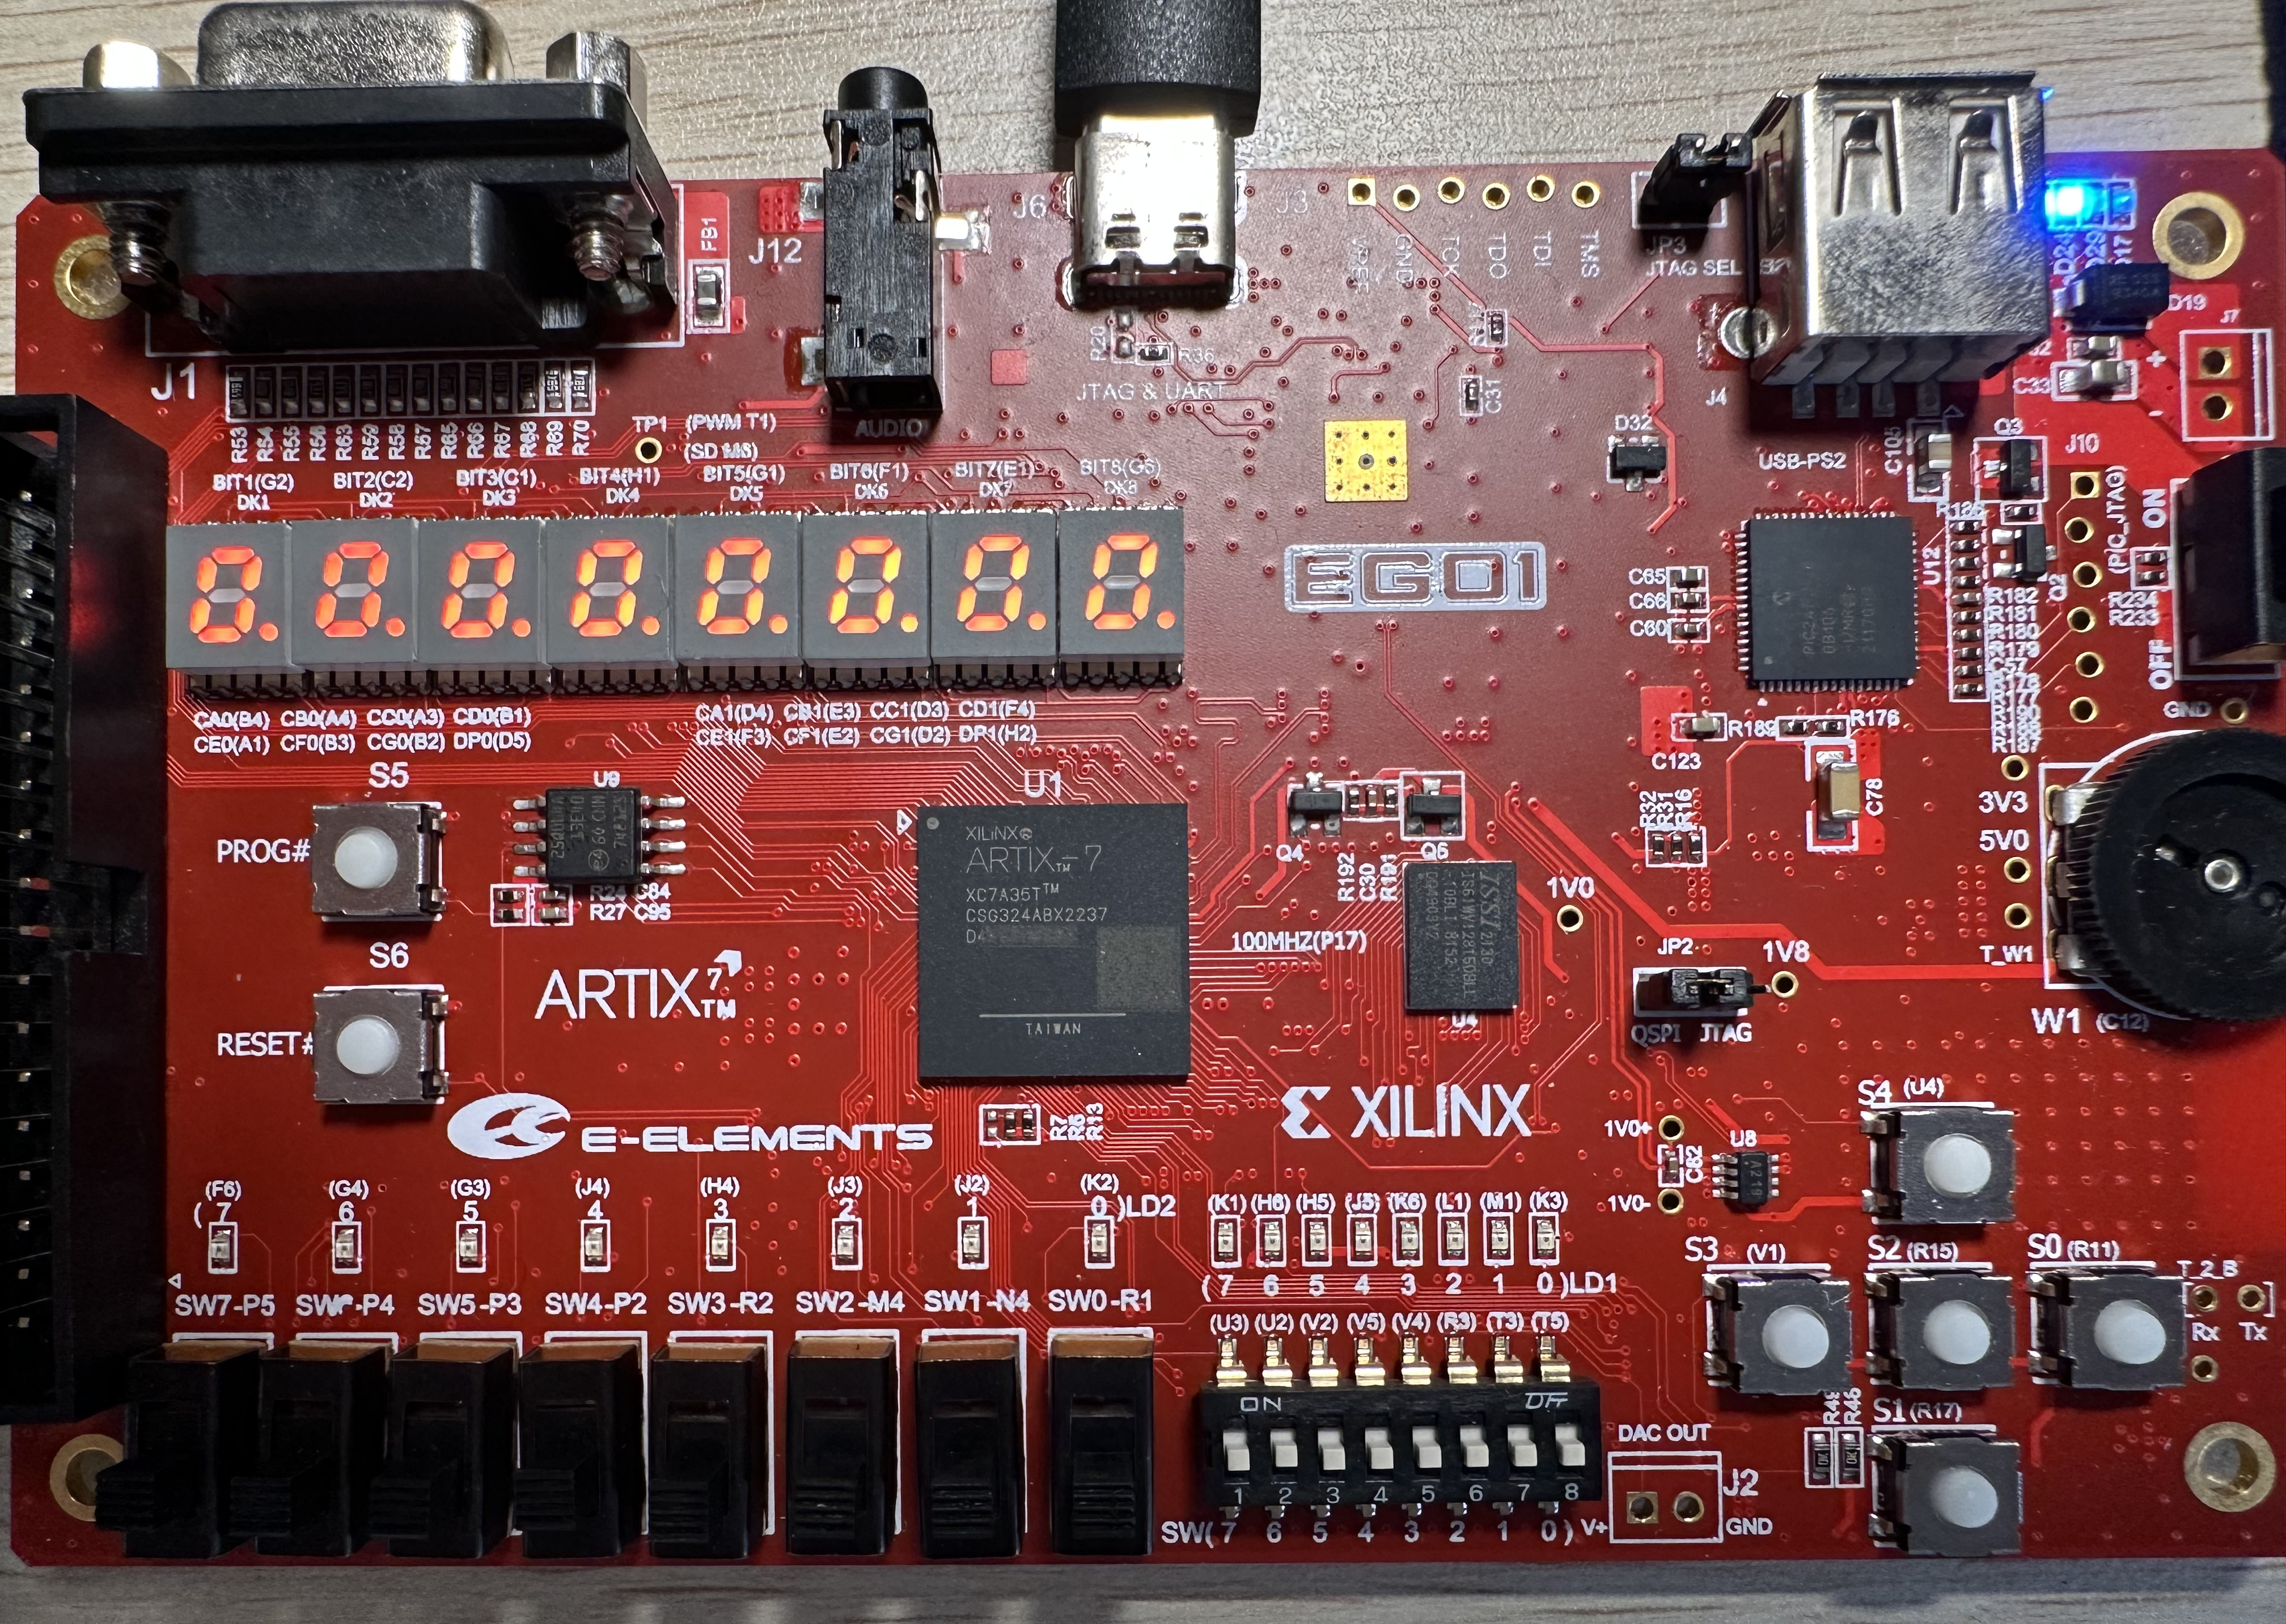
\includegraphics[width=0.6\textwidth]{images/origin.png}
  \caption{实验所用 FPGA 开发板示意图}
  \label{fig:origin.png}
\end{figure}

本实验采用EGO1开发板进行板级验证,通过管脚约束将硬件I/O端口与逻辑信号建立映射:输入端利用板载拨码开关设定内存地址,

控制信号\texttt{clkreset}、\texttt{reset} 及 \texttt{enable} 被分配至指定拨码开关,而\texttt{start}与\texttt{read}信号则由按键触发 ;

\begin{center}
\begin{tikzpicture}[every node/.style={font=\small, inner sep=1pt}]

    % 1. 绘制8个数码管位 (总宽约 10cm)
    % 调整了矩形大小和间距以适应 small 字体
    \foreach \i in {0,...,7} {
        % 间距系数设为 1.2,方框宽 1.0
        \draw[fill=blue!10] (\i*1.2, 0) rectangle (\i*1.2+1.0, 1.2);
        % 在方框内画一个简单的 "8." 示意图
        \node[gray!50] at (\i*1.2+0.5, 0.6) {\textbf{8.}};
    }

    % 2. 顶部标号 (数码管索引)
    \foreach \i/\label in {0/7, 1/6, 2/5, 3/4, 4/3, 5/2, 6/1, 7/0} {
        \node[above] at (\i*1.2+0.5, 1.2) {D \label};
    }

    % 3. 顶部分组说明 (Hex模式下的 PC码 和 内存数据)
    % 高四位 (左边4个: 索引0-3, 坐标范围 0 到 3*1.2+1.0 = 4.6)
    \draw [decorate,decoration={brace,amplitude=5pt},thick] (0, 1.7) -- (4.6, 1.7) 
        node[midway,above=5pt] {\textbf{PC 指针代码} (高4位)};
    
    % 低四位 (右边4个: 索引4-7, 坐标范围 4.8 到 7*1.2+1.0 = 9.4)
    \draw [decorate,decoration={brace,amplitude=5pt},thick] (4.8, 1.7) -- (9.4, 1.7) 
        node[midway,above=5pt] {\textbf{内存数据} (低4位)};

    % 图标题
    \node[align=center, blue] at (4.7, 3.0) {\large \textbf{输出显示逻辑分配 (十六进制模式)}};

\end{tikzpicture}
\end{center}

输出端利用8位七段数码管实时监测系统状态,并根据实验需求设计了十六进制与十进制两种显示模式,在十六进制模式下,数码管高四位用于显示PC码,低四位显示内存数据,十进制模式则相应调整位宽分配以呈现对应的十进制数值;系统设有严格的启动时序保护,\textbf{当且仅当\texttt{clkreset}信号置为低电平(0),且\texttt{reset}、\texttt{enable}及\texttt{start}信号均置为高电平(1)时,流水线处理器方进入执行状态},数码管随即启动并实时更新显示当前的PC地址与内存数据。


\begin{center}
% =========================================
% 图2:系统启动时序保护
% =========================================
\begin{tikzpicture}[scale=1, every node/.style={font=\small, inner sep=2pt}]

    % 1. 绘制信号输入节点
    % 增加垂直间距以适应字体
    \node[right] at (-1, 2.4) {\texttt{clkreset}};
    \node[right] at (-1, 1.6) {\texttt{reset}};
    \node[right] at (-1, 0.8) {\texttt{enable}};
    \node[right] at (-1, 0.0) {\texttt{start}};

    % 信号电平要求
    \draw[fill=red!10] (2.5, 2.4) circle (0.35) node {0}; % 低电平
    \draw[fill=green!10] (2.5, 1.6) circle (0.35) node {1}; % 高电平
    \draw[fill=green!10] (2.5, 0.8) circle (0.35) node {1}; % 高电平
    \draw[fill=green!10] (2.5, 0.0) circle (0.35) node {1}; % 高电平

    % 连接线
    \draw[->, thick] (1.0, 2.4) -- (2.1, 2.4);
    \draw[->, thick] (1.0, 1.6) -- (2.1, 1.6);
    \draw[->, thick] (1.0, 0.8) -- (2.1, 0.8);
    \draw[->, thick] (1.0, 0.0) -- (2.1, 0.0);

    % 2. 逻辑判定框 (AND Logic)
    % 放大判定框
    \draw[fill=blue!10, rounded corners=5pt] (4, -0.5) rectangle (7, 3.0);
    \node[align=center] at (5.5, 1.25) {与逻辑\\(AND)};

    % 连接信号到逻辑框
    \draw (2.85, 2.4) -- (4, 2.4);
    \draw (2.85, 1.6) -- (4, 1.6);
    \draw (2.85, 0.8) -- (4, 0.8);
    \draw (2.85, 0.0) -- (4, 0.0);

    % 3. 输出结果
    \draw[->, thick, ultra thick] (7, 1.25) -- (8.5, 1.25);
    
    % 结果状态框
    \draw[fill=orange!10] (8.5, 0.0) rectangle (12.5, 2.5);
    \node[align=center, text width=3.5cm] at (10.5, 1.25) {
        \textbf{系统状态: 执行}\\
        1. 流水线启动\\
        2. 数码管实时更新
    };

    % 图标题
    \node[align=center, blue] at (5.5, 4.0) {\large \textbf{系统启动时序保护逻辑}};

\end{tikzpicture}
\end{center}

\subsubsection{全指令测试}

\noindent
\begin{minipage}{0.32\textwidth}
  \centering
  \includegraphics[width=\linewidth]{images/1-1.jpg}
  
  \texttt{ADD:00000016,CELL:fffe}
\end{minipage}
\hfill
\begin{minipage}{0.32\textwidth}
  \centering
  \includegraphics[width=\linewidth]{images/1-2.jpg}
  
  \texttt{ADD:00000004,CELL:69c3}
\end{minipage}
\hfill
\begin{minipage}{0.32\textwidth}
  \centering
  \includegraphics[width=\linewidth]{images/1-3.jpg}

  \texttt{PC:6AH=106D};数据 \texttt{69c3H=27075D}
\end{minipage}

\texttt{PC=106D} 对应 \texttt{I\_mem} 中 \texttt{HALT} 的下一条指令地址:由于 \texttt{HALT} 进入 \texttt{id\_ir} 时,PC 自增并指向下一条指令(即 $105+1=106$)


\noindent
\begin{minipage}{0.3\textwidth}

\begin{lstlisting}[language=bash]
ADD:00000000,CELL:fffd
ADD:00000001,CELL:0004
ADD:00000002,CELL:0005
ADD:00000003,CELL:c369
ADD:00000004,CELL:69c3
ADD:00000005,CELL:0041
ADD:00000006,CELL:ffff
ADD:00000007,CELL:0001
ADD:00000008,CELL:0000
ADD:00000009,CELL:0000
ADD:0000000a,CELL:0000
ADD:0000000b,CELL:xxxx
ADD:0000000c,CELL:xxxx
ADD:0000000d,CELL:xxxx
ADD:0000000e,CELL:xxxx
ADD:0000000f,CELL:xxxx
ADD:00000010,CELL:b600
\end{lstlisting}

\end{minipage}
\hfill
\begin{minipage}{0.3\textwidth}
\begin{lstlisting}[language=bash]
ADD:00000011,CELL:0001
ADD:00000012,CELL:0005
ADD:00000013,CELL:0001
ADD:00000014,CELL:ffff
ADD:00000015,CELL:fffe
ADD:00000016,CELL:fffe
ADD:00000017,CELL:fffe
ADD:00000018,CELL:fffe
ADD:00000019,CELL:c369
ADD:0000001a,CELL:86d2
ADD:0000001b,CELL:3690
ADD:0000001c,CELL:8000
ADD:0000001d,CELL:c369
ADD:0000001e,CELL:61b4
ADD:0000001f,CELL:00c3
ADD:00000020,CELL:0001
\end{lstlisting}

\end{minipage}
\hfill
\begin{minipage}{0.3\textwidth}

\begin{lstlisting}[language=bash]
ADD:00000021,CELL:c369
ADD:00000022,CELL:86d2
ADD:00000023,CELL:6900
ADD:00000024,CELL:8000
ADD:00000025,CELL:69c3
ADD:00000026,CELL:d386
ADD:00000027,CELL:c300
ADD:00000028,CELL:8000
ADD:00000029,CELL:c369
ADD:0000002a,CELL:61b4
ADD:0000002b,CELL:00c3
ADD:0000002c,CELL:0001
ADD:0000002d,CELL:69c3
ADD:0000002e,CELL:34e1
ADD:0000002f,CELL:0069
ADD:00000030,CELL:0000
\end{lstlisting}

\end{minipage}

\subsubsection{最大公约数、最小公倍数算法验证}

\noindent
\begin{minipage}{0.32\textwidth}
  \centering
  \includegraphics[width=\linewidth]{images/2-1.jpg}
  
  \texttt{ADD:00000003,CELL:0008}
\end{minipage}
\hfill
\begin{minipage}{0.32\textwidth}
  \centering
  \includegraphics[width=\linewidth]{images/2-2.jpg}
  
  \texttt{ADD:00000002,CELL:0018}
\end{minipage}
\hfill
\begin{minipage}{0.32\textwidth}
  \centering
  \includegraphics[width=\linewidth]{images/2-3.jpg}

  \texttt{PC:18H=24D};数据 \texttt{0018H=0024D}
\end{minipage}

\texttt{PC=24D} 对应着 \texttt{I\_mem} 中 \texttt{HALT} 指令下一条指令的地址,即下一条指令的地址 \texttt{24D}

\begin{lstlisting}[language=bash]
ADD:00000000,CELL:0000
ADD:00000001,CELL:0020
ADD:00000002,CELL:0018
ADD:00000003,CELL:0008
ADD:00000004,CELL:0060
\end{lstlisting}

\subsubsection{64 位加法验证}

\noindent
\begin{minipage}{0.32\textwidth}
  \centering
  \includegraphics[width=\linewidth]{images/3-1.jpg}
  
  \texttt{ADD:00000002,CELL:fffe}
\end{minipage}
\hfill
\begin{minipage}{0.32\textwidth}
  \centering
  \includegraphics[width=\linewidth]{images/3-2.jpg}
  
  \texttt{ADD:00000008,CELL:fffd}
\end{minipage}
\hfill
\begin{minipage}{0.32\textwidth}
  \centering
  \includegraphics[width=\linewidth]{images/3-3.jpg}

  \texttt{PC:13H=19D};数据 \texttt{fffdH=65533D}
\end{minipage}

\texttt{PC=19D} 对应着 \texttt{I\_mem} 中 \texttt{HALT} 指令下一条指令的地址 \texttt{19D}

\begin{lstlisting}[language=bash]
ADD:00000000,CELL:fffe
ADD:00000001,CELL:fffe
ADD:00000002,CELL:fffe
ADD:00000003,CELL:0000
ADD:00000004,CELL:ffff
ADD:00000005,CELL:ffff
ADD:00000006,CELL:ffff
ADD:00000007,CELL:0000
ADD:00000008,CELL:fffd
ADD:00000009,CELL:fffe
ADD:0000000a,CELL:fffe
ADD:0000000b,CELL:0001
\end{lstlisting}

\subsubsection{冒泡排序算法测试}

\noindent
\begin{minipage}{0.32\textwidth}
  \centering
  \includegraphics[width=\linewidth]{images/4-1.jpg}
  
  \texttt{ADD:00000002,CELL:6152}
\end{minipage}
\hfill
\begin{minipage}{0.32\textwidth}
  \centering
  \includegraphics[width=\linewidth]{images/4-2.jpg}
  
  \texttt{ADD:00000008,CELL:0060}
\end{minipage}
\hfill
\begin{minipage}{0.32\textwidth}
  \centering
  \includegraphics[width=\linewidth]{images/4-3.jpg}

  \texttt{PC:11H=17D};数据 \texttt{2369H=09065D}
\end{minipage}

\texttt{PC=17D} 对应着 \texttt{I\_mem} 中 \texttt{HALT} 指令下一条指令的地址 \texttt{17D}

\begin{lstlisting}[language=bash]
ADD:00000000,CELL:000a
ADD:00000001,CELL:69c3
ADD:00000002,CELL:6152
ADD:00000003,CELL:5555
ADD:00000004,CELL:2895
ADD:00000005,CELL:2369
ADD:00000006,CELL:1057
ADD:00000007,CELL:0fff
ADD:00000008,CELL:0060
ADD:00000009,CELL:0005
ADD:0000000a,CELL:0004
ADD:0000000b,CELL:0000
\end{lstlisting}

\subsubsection{sort 排序算法测试}

\noindent
\begin{minipage}{0.32\textwidth}
  \centering
  \includegraphics[width=\linewidth]{images/5-1.jpg}
  
  \texttt{ADD:00000002,CELL:0001}
\end{minipage}
\hfill
\begin{minipage}{0.32\textwidth}
  \centering
  \includegraphics[width=\linewidth]{images/5-2.jpg}
  
  \texttt{ADD:00000008,CELL:000a}
\end{minipage}
\hfill
\begin{minipage}{0.32\textwidth}
  \centering
  \includegraphics[width=\linewidth]{images/5-3.jpg}

  \texttt{PC:13H=19D};数据 \texttt{000aH=00010D}
\end{minipage}

\texttt{PC=19D} 也正好对应着 \texttt{I\_mem} 中 \texttt{HALT} 指令下一条指令的地址 \texttt{19D}

\begin{lstlisting}[language=bash]
ADD:00000000,CELL:0000
ADD:00000001,CELL:0000
ADD:00000002,CELL:0001
ADD:00000003,CELL:0003
ADD:00000004,CELL:0004
ADD:00000005,CELL:0005
ADD:00000006,CELL:0006
ADD:00000007,CELL:0009
ADD:00000008,CELL:000a
ADD:00000009,CELL:0011
\end{lstlisting}

% 总结
\section{总结}

本实验完成了流水线 MIPS 处理器的关键模块补全与系统级验证。首先在 ID 阶段加入基于 EX/MEM/WB 三级的前递判定逻辑,实现对算术/逻辑/移位/立即数以及 \texttt{LOAD} 等指令的数据相关处理,尽量在不插入气泡的情况下消除数据冒险;随后补全 ALU 的各类运算与地址计算路径,保证控制信号与运算结果在流水线各级之间传递一致。

在验证环节,编写 testbench 生成时钟与复位序列,按照启动时序对 CPU 进行使能运行,并通过转储 \texttt{d\_mem} 的方式对执行结果进行对比检查。仿真结果表明处理器能够正确执行全指令集测试、最大公约数/最小公倍数求解、64 位加法以及冒泡排序等程序,说明前递逻辑与 ALU 运算功能满足设计要求。

在板级验证部分,完成 XDC 管脚约束与数码管显示链路设计,将 PC 与数据存储器内容以十进制方式输出,便于观察运行状态与最终结果。总体上,本实验加深了对流水线结构、数据/控制冒险来源及其解决方法(前递、必要时停顿)的理解,并熟悉了从模块实现、仿真验证到 FPGA 约束与板级观测的完整硬件开发流程。

\appendix
\renewcommand{\thesection}{附录\Alph{section}}

\section{\texttt{test.v}代码}

\begin{lstlisting}[language=Verilog]
`timescale 1ps / 1ps
module test;

  // inputs
  reg clk;
  reg enable;
  reg reset;
  reg start;
  reg read;
  reg [7:0] adress;
  reg clkreset;

  // outputs
  wire [6:0] light;
  wire [3:0] an;
  wire [6:0] light2;
  wire [3:0] an2;

  integer x;

  // UUT
  cpu uut (
    .clk(clk),
    .enable(enable),
    .reset(reset),
    .read(read),
    .clkreset(clkreset),
    .start(start),
    .adress(adress),
    .light(light),
    .an(an),
    .light2(light2),
    .an2(an2)
  );

  // clocks
  always #1  clk      = ~clk;
  always #20 clkreset = ~clkreset;

  initial begin
    // init
    clk      = 1'b0;
    clkreset = 1'b0;
    enable   = 1'b0;
    start    = 1'b0;
    read     = 1'b0;
    adress   = 8'h00;
    x        = 0;

    // reset (active low)
    reset = 1'b0;
    repeat (5) @(posedge clk);
    reset = 1'b1;

    // enable + start
    repeat (2) @(posedge clk);
    enable = 1'b1;
    start  = 1'b1;

    // run
    repeat (2000) @(posedge clk);

    // dump d_mem
    read = 1'b0;
    x = 0;
    repeat (65) begin
      $display("ADD:%h,CELL:%h", x, uut.d_mem.d_mem[x]);
      x = x + 1;
    end

    $finish;
  end

endmodule
\end{lstlisting}

\section{管脚约束代码}

\begin{lstlisting}[language=Verilog]
# 给下半片4个数码管的段选输出信号分配电平
set_property IOSTANDARD LVCMOS33 [get_ports {light[6]}]
set_property IOSTANDARD LVCMOS33 [get_ports {light[5]}]
set_property IOSTANDARD LVCMOS33 [get_ports {light[4]}]
set_property IOSTANDARD LVCMOS33 [get_ports {light[3]}]
set_property IOSTANDARD LVCMOS33 [get_ports {light[2]}]
set_property IOSTANDARD LVCMOS33 [get_ports {light[1]}]
set_property IOSTANDARD LVCMOS33 [get_ports {light[0]}]

# 给下半片4个数码管的段选输出信号分配接口
set_property PACKAGE_PIN D4 [get_ports {light[6]}]
set_property PACKAGE_PIN D3 [get_ports {light[4]}]
set_property PACKAGE_PIN E3 [get_ports {light[5]}]
set_property PACKAGE_PIN F4 [get_ports {light[3]}]
set_property PACKAGE_PIN F3 [get_ports {light[2]}]
set_property PACKAGE_PIN E2 [get_ports {light[1]}]
set_property PACKAGE_PIN D2 [get_ports {light[0]}]

# 给上半片4个数码管的段选输出信号分配电平
set_property IOSTANDARD LVCMOS33 [get_ports {light2[6]}]
set_property IOSTANDARD LVCMOS33 [get_ports {light2[5]}]
set_property IOSTANDARD LVCMOS33 [get_ports {light2[4]}]
set_property IOSTANDARD LVCMOS33 [get_ports {light2[3]}]
set_property IOSTANDARD LVCMOS33 [get_ports {light2[2]}]
set_property IOSTANDARD LVCMOS33 [get_ports {light2[1]}]
set_property IOSTANDARD LVCMOS33 [get_ports {light2[0]}]

# 给上半片4个数码管的段选输出信号分配接口
set_property PACKAGE_PIN B4 [get_ports {light2[6]}]
set_property PACKAGE_PIN A4 [get_ports {light2[5]}]
set_property PACKAGE_PIN A3 [get_ports {light2[4]}]
set_property PACKAGE_PIN B1 [get_ports {light2[3]}]
set_property PACKAGE_PIN A1 [get_ports {light2[2]}]
set_property PACKAGE_PIN B3 [get_ports {light2[1]}]
set_property PACKAGE_PIN B2 [get_ports {light2[0]}]
\end{lstlisting}

\begin{lstlisting}[language=Verilog]
# 给下半片4个数码管的位选输出信号分配电平
set_property IOSTANDARD LVCMOS33 [get_ports {an[3]}]
set_property IOSTANDARD LVCMOS33 [get_ports {an[2]}]
set_property IOSTANDARD LVCMOS33 [get_ports {an[1]}]
set_property IOSTANDARD LVCMOS33 [get_ports {an[0]}]

# 给下半片4个数码管的位选输出信号分配接口
set_property PACKAGE_PIN G1 [get_ports {an[3]}]
set_property PACKAGE_PIN F1 [get_ports {an[2]}]
set_property PACKAGE_PIN E1 [get_ports {an[1]}]
set_property PACKAGE_PIN G6 [get_ports {an[0]}]

# 给上半片4个数码管的位选输出信号分配电平
set_property IOSTANDARD LVCMOS33 [get_ports {an2[3]}]
set_property IOSTANDARD LVCMOS33 [get_ports {an2[2]}]
set_property IOSTANDARD LVCMOS33 [get_ports {an2[1]}]
set_property IOSTANDARD LVCMOS33 [get_ports {an2[0]}]

# 给上半片4个数码管的位选输出信号分配接口
set_property PACKAGE_PIN G2 [get_ports {an2[3]}]
set_property PACKAGE_PIN C2 [get_ports {an2[2]}]
set_property PACKAGE_PIN C1 [get_ports {an2[1]}]
set_property PACKAGE_PIN H1 [get_ports {an2[0]}]

# 给D_mem的输入地址信号分配电平
set_property IOSTANDARD LVCMOS33 [get_ports {address[7]}]
set_property IOSTANDARD LVCMOS33 [get_ports {address[6]}]
set_property IOSTANDARD LVCMOS33 [get_ports {address[5]}]
set_property IOSTANDARD LVCMOS33 [get_ports {address[4]}]
set_property IOSTANDARD LVCMOS33 [get_ports {address[3]}]
set_property IOSTANDARD LVCMOS33 [get_ports {address[2]}]
set_property IOSTANDARD LVCMOS33 [get_ports {address[1]}]
set_property IOSTANDARD LVCMOS33 [get_ports {address[0]}]
\end{lstlisting}

\begin{lstlisting}[language=Verilog]
# 给D_mem的输入地址信号分配接口
set_property PACKAGE_PIN P5 [get_ports {adress[7]}]
set_property PACKAGE_PIN P4 [get_ports {adress[6]}]
set_property PACKAGE_PIN P3 [get_ports {adress[5]}]
set_property PACKAGE_PIN P2 [get_ports {adress[4]}]
set_property PACKAGE_PIN R2 [get_ports {adress[3]}]
set_property PACKAGE_PIN M4 [get_ports {adress[2]}]
set_property PACKAGE_PIN N4 [get_ports {adress[1]}]
set_property PACKAGE_PIN R1 [get_ports {adress[0]}]

# 给全局时钟输入信号分配分配电平和接口
set_property IOSTANDARD LVCMOS33 [get_ports clk]
set_property PACKAGE_PIN P17 [get_ports clk]

# 给enable输入信号分配分配电平和接口
set_property IOSTANDARD LVCMOS33 [get_ports enable]
set_property PACKAGE_PIN T5 [get_ports enable]

# 给reset输入信号分配分配电平和接口
set_property IOSTANDARD LVCMOS33 [get_ports reset]
set_property PACKAGE_PIN T3 [get_ports reset]

# 给read输入信号分配分配电平和接口
set_property IOSTANDARD LVCMOS33 [get_ports read]
set_property PACKAGE_PIN R11 [get_ports read]
\end{lstlisting}

\begin{lstlisting}[language=Verilog]
# 给reset输入信号分配配电平和接口
set_property IOSTANDARD LVCMOS33 [get_ports clkreset]
set_property PACKAGE_PIN R3 [get_ports clkreset]

# 给start输入信号分配配电平和接口
set_property IOSTANDARD LVCMOS33 [get_ports start]
set_property PACKAGE_PIN R17 [get_ports start]

# 给出综合需要用到的时钟信号
create_clock -period 11.000 -name clk -waveform {0.000 5.500} [get_ports clk]
set_input_delay -clock [get_clocks clk] -min -add_delay 0.000 [get_ports {adress[*]}]
set_input_delay -clock [get_clocks clk] -max -add_delay 0.000 [get_ports {adress[*]}]
set_input_delay -clock [get_clocks clk] -min -add_delay 0.000 [get_ports clkreset]
set_input_delay -clock [get_clocks clk] -max -add_delay 0.000 [get_ports clkreset]
set_input_delay -clock [get_clocks clk] -min -add_delay 0.000 [get_ports read]
set_input_delay -clock [get_clocks clk] -max -add_delay 0.000 [get_ports read]
set_output_delay -clock [get_clocks clk] -min -add_delay 0.000 [get_ports {an[*]}]
set_output_delay -clock [get_clocks clk] -max -add_delay 0.000 [get_ports {an[*]}]
set_output_delay -clock [get_clocks clk] -min -add_delay 0.000 [get_ports {an2[*]}]
set_output_delay -clock [get_clocks clk] -max -add_delay 0.000 [get_ports {an2[*]}]
set_output_delay -clock [get_clocks clk] -min -add_delay 0.000 [get_ports {light[*]}]
set_output_delay -clock [get_clocks clk] -max -add_delay 0.000 [get_ports {light[*]}]
set_output_delay -clock [get_clocks clk] -min -add_delay 0.000 [get_ports {light2[*]}]
set_output_delay -clock [get_clocks clk] -max -add_delay 0.000 [get_ports {light2[*]}]
\end{lstlisting}

\section{十进制显示译码器代码}

\begin{lstlisting}[language=Verilog]
module decoder10(
    input clock,
    input reset,
    input [15:0] y,     // 接dmen四位16进制输入
    output reg [6:0] select_segment,
    output reg [3:0] select_bit,
    output [3:0] BCDout // 输出BCD码最高位
);

wire [1:0] s;
reg [3:0] digit;
reg [20:0] clkdiv;
wire [15:0] BCD;

assign s = clkdiv[20:19];
assign BCDout[3:0] = (y/10000)%10;   // D_mem码万位数
assign BCD[15:12] = (y/1000)%10;     // D_mem码千位数
assign BCD[11:8] = (y/100)%10;       // D_mem码百位数
assign BCD[7:4] = (y/10)%10;         // D_mem码十位数
assign BCD[3:0] = y%10;              // D_mem码个位数

always @(posedge clock) begin
    case(s)
        0: digit = BCD[3:0];
        1: digit = BCD[7:4];
        2: digit = BCD[11:8];
        3: digit = BCD[15:12];
        default: digit = BCD[3:0];
    endcase
end

always @(posedge clock) begin
    case(digit)    // 十六进制输出
        0: select_segment = 7'b1111_110;  // 0
        1: select_segment = 7'b0110_000;  // 1
        2: select_segment = 7'b1101_101;  // 2
        3: select_segment = 7'b1111_001;  // 3
        4: select_segment = 7'b0110_011;  // 4
        5: select_segment = 7'b1011_011;  // 5
        6: select_segment = 7'b1011_111;  // 6
        7: select_segment = 7'b1110_000;  // 7
        8: select_segment = 7'b1111_111;  // 8
        9: select_segment = 7'b1111_011;  // 9
    endcase
end

always @(posedge clock) begin
    case(clkdiv[1:0])
        0: select_bit = 4'b0001;  // 消除显影
        1: select_bit = 4'b0010;  // 指定s位位选
        2: select_bit = 4'b0100;
        3: select_bit = 4'b1000;
    endcase
end

always @(posedge clock or posedge reset) begin
    if (reset) begin
        clkdiv <= 0;
    end
    else begin
        clkdiv <= clkdiv + 1;
    end
end

endmodule
\end{lstlisting}

\begin{lstlisting}[language=Verilog]
module decoder10_2(
    input clock,
    input reset,
    input [15:0] y,     // 接PC码输入
    input [3:0] BCDin,  // 接dmen最高位BCD码
    output reg [6:0] select_segment,
    output reg [3:0] select_bit
);

wire [1:0] s;
reg [3:0] digit;
reg [20:0] clkdiv;
wire [11:0] BCD;

assign s = clkdiv[20:19];
assign BCD[11:8] = y/100;     // PC码百位数
assign BCD[7:4] = (y/10)%10;  // PC码十位数
assign BCD[3:0] = y%10;       // PC码个位数

always @(posedge clock) begin
    case(s)
        0: digit = BCDin[3:0];
        1: digit = BCD[3:0];
        2: digit = BCD[7:4];
        3: digit = BCD[11:8];
        default: digit = BCD[3:0];
    endcase
end

always @(posedge clock) begin
    case(digit)  // 十六进制输出
        0: select_segment = 7'b1111110;  // 0
        1: select_segment = 7'b0110000;  // 1
        2: select_segment = 7'b1101101;  // 2
        3: select_segment = 7'b1111001;  // 3
        4: select_segment = 7'b0110011;  // 4
        5: select_segment = 7'b1011011;  // 5
        6: select_segment = 7'b1011111;  // 6
        7: select_segment = 7'b1110000;  // 7
        8: select_segment = 7'b1111111;  // 8
        9: select_segment = 7'b1111011;  // 9
        default: select_segment = 7'b1111110;  // 0
    endcase
end

endmodule
\end{lstlisting}

\end{document}